\documentclass{article}

\usepackage{graphicx}
\usepackage{tikz}
\usepackage{tikzsymbols}
\usetikzlibrary{calc,patterns,shapes.geometric}
\pagestyle{empty}
\usepackage[margin=0pt]{geometry}
\geometry{papersize={14in,12in}}

\def\centerarc[#1](#2)(#3:#4:#5){\draw[#1] ($(#2)+({#5*cos(#3)},{#5*sin(#3)})$) arc (#3:#4:#5);}

\begin{document}
	\begin{figure}
		\centering
		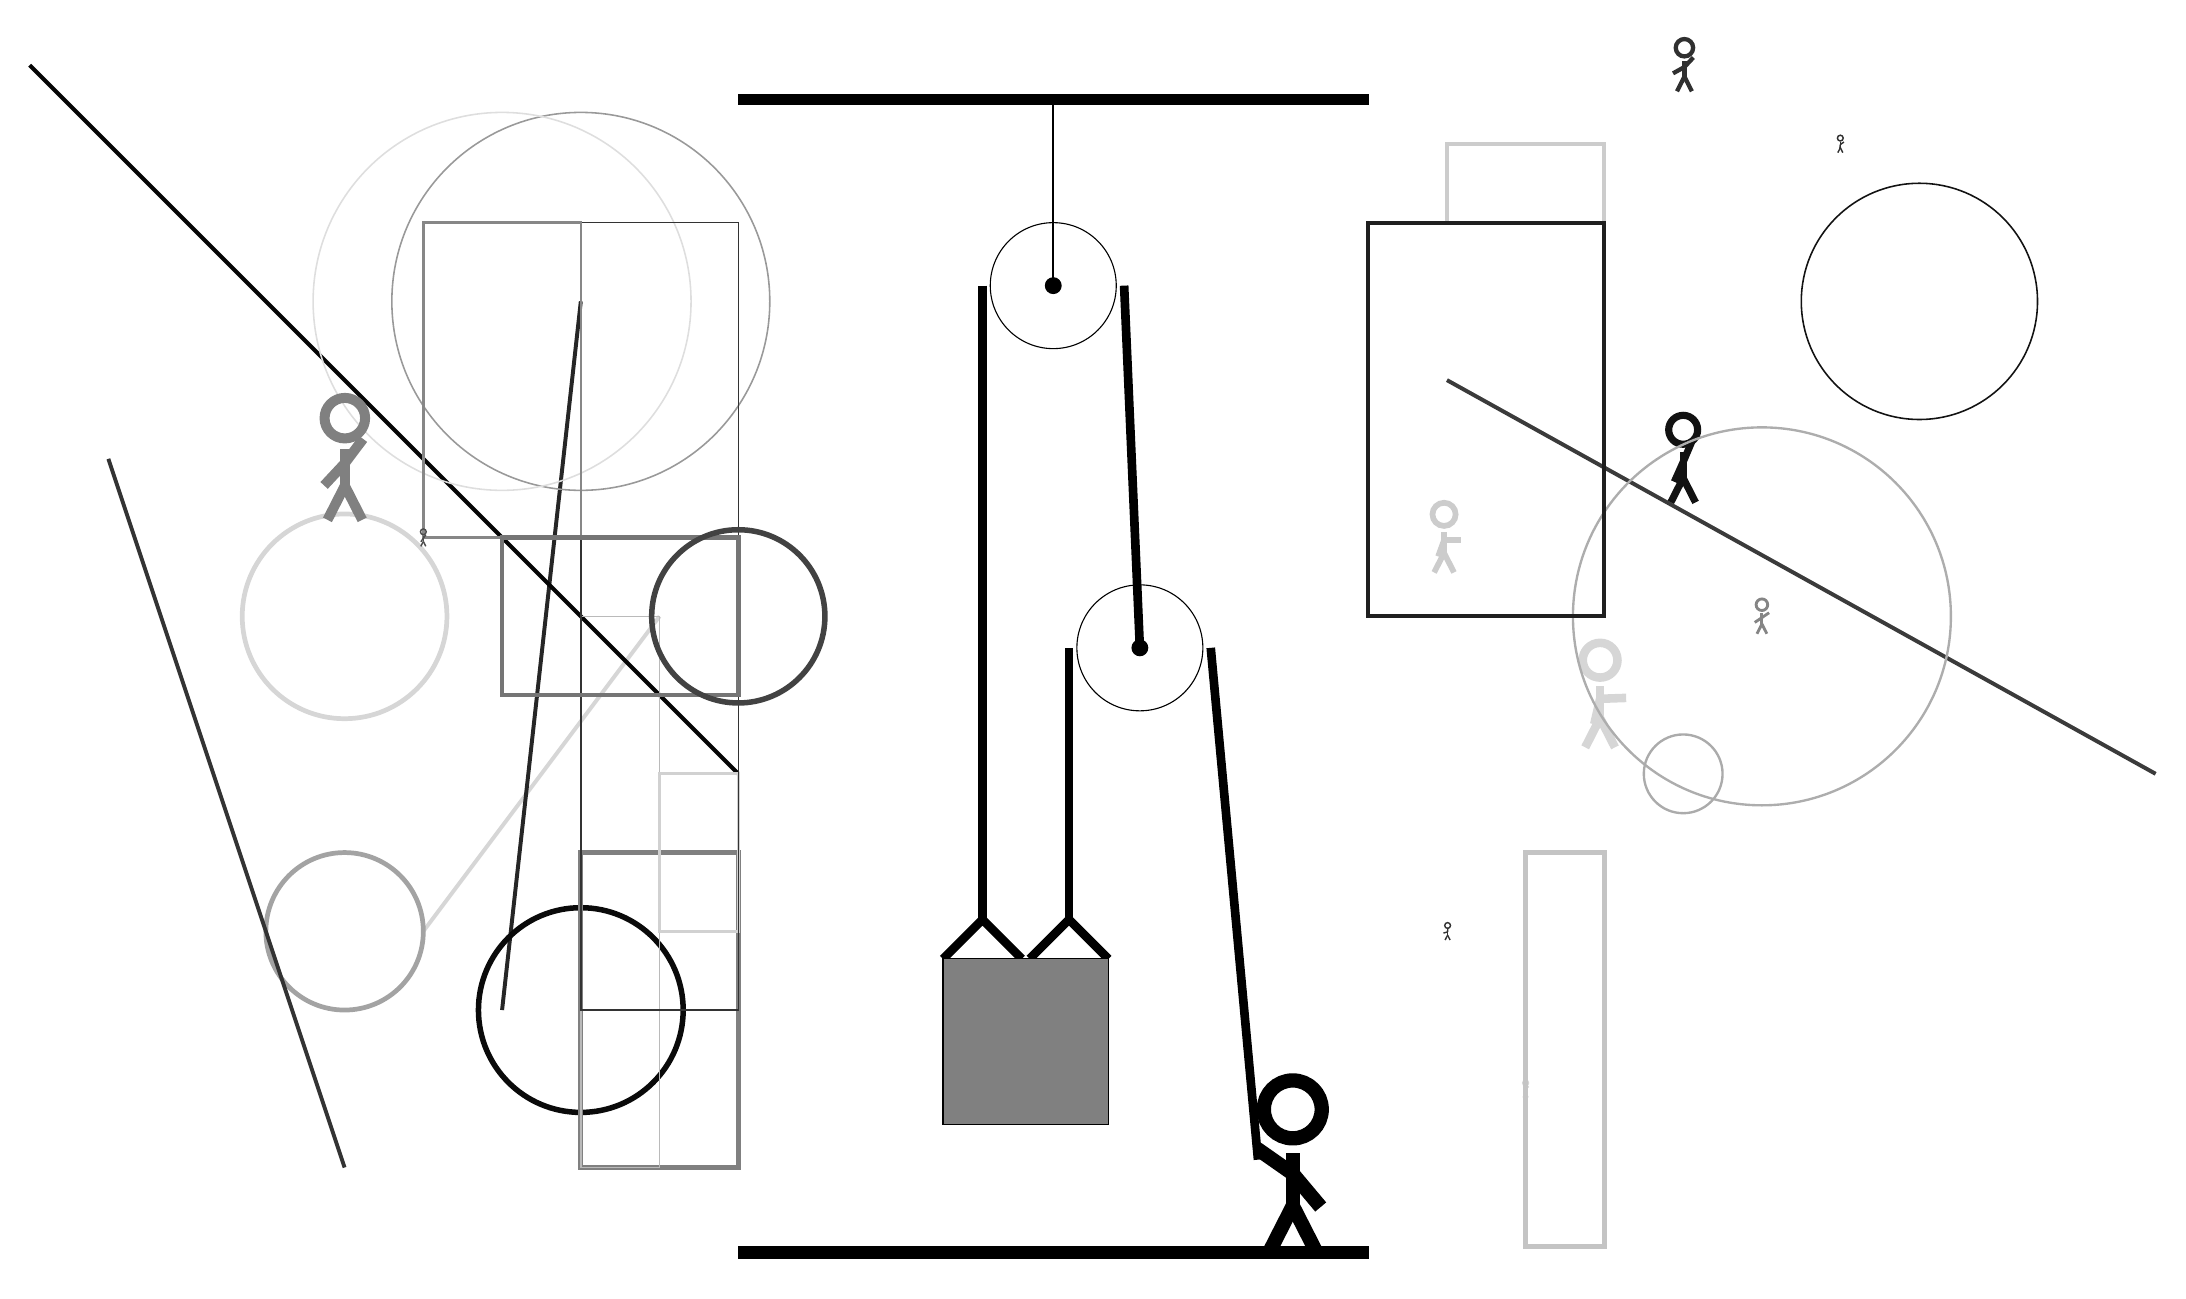
\begin{tikzpicture}
			%%%%% START %%%%%
			
			\draw[fill=black] (-2, 11.5) rectangle (6, 11.625);
			
			\node[line width=0.2mm, color=black!16] at (9, 4) {\Strichmaxerl[6][77][2]};
			
			\draw[line width=0.5mm, color=black!16](-3, 5) -- (-6, 1);
			\draw[line width=0.5mm, color=black!85](-5, 0) -- (-4, 9);
			\draw[line width=0.5mm, color=black!98](-2, 3) -- (-11, 12);
			\draw [line width=0.7mm, color=black!96](-4, 0) circle (1.3);
			
			\node[line width=0.3mm, color=black!93] at (10, 7) {\Strichmaxerl[5][66][67]};
			
			\node[line width=0.2mm, color=black!20] at (7, 6) {\Strichmaxerl[4][70][0]};
			
			\node[line width=0.2mm, color=black!17] at (8, -1) {\Strichmaxerl[1][83][45]};
			\draw [line width=0.6mm, color=black!36](-7, 1) circle (1.0);
			\draw[line width=0.5mm, color=black!20] (7, 11) rectangle (9, 10);
			\draw[line width=0.6mm, color=black!50] (-4, -2) rectangle (-2, 2);
			
			\draw[line width=0.5mm, color=black!80](-7, -2) -- (-10, 7);
			\draw[line width=0.5mm, color=black!77](7, 8) -- (16, 3);
			\draw [line width=0.3mm, color=black!32](11, 5) circle (2.4);
			\draw [line width=0.2mm, color=black!93](13, 9) circle (1.5);
			\draw [line width=0.2mm, color=black!40](-4, 9) circle (2.4);
			\draw [line width=0.6mm, color=black!16](-7, 5) circle (1.3);
			\draw[line width=0.2mm, color=black!27] (-3, 5) rectangle (-4, -2);
			\node[line width=0.7mm, color=black!48] at (11, 5) {\Strichmaxerl[2][34][34]};
			\draw [line width=0.2mm, color=black!13](-5, 9) circle (2.4);
			\draw[line width=0.5mm, color=black!88] (6, 5) rectangle (9, 10);
			
			\draw[line width=0.4mm, color=black!18] (-3, 1) rectangle (-2, 3);
			\draw[line width=0.2mm, color=black!80] (-4, 0) rectangle (-2, 10);
			\draw[line width=0.6mm, color=black!23] (8, 2) rectangle (9, -3);
			\node[line width=0.6mm, color=black!81] at (10, 12) {\Strichmaxerl[3][29][47]};
			\draw[line width=0.3mm, color=black!47] (-4, 10) rectangle (-6, 6);
			
			\draw[line width=0.6mm, color=black!54] (-2, 6) rectangle (-5, 4);
			\node[line width=0.3mm, color=black!50] at (-7, 7) {\Strichmaxerl[7][47][53]};
			\node[line width=0.2mm, color=black!70] at (-6, 6) {\Strichmaxerl[1][55][54]};
			\node[line width=0.2mm, color=black!80] at (7, 1) {\Strichmaxerl[1][15][87]};
			\draw [line width=0.3mm, color=black!33](10, 3) circle (0.5);
			
			\node[line width=0.5mm, color=black!81] at (12, 11) {\Strichmaxerl[1][83][35]};
			\draw [line width=0.7mm, color=black!74](-2, 5) circle (1.1);
			
			\draw (2, 9.2) circle (0.8);
			\draw[fill=black] (2, 9.2) circle (0.1);
			\draw[thick] (2, 9.2) -- (2, 11.5);
			
			\draw (3.1, 4.6) circle (0.8);
			\draw[fill=black] (3.1, 4.6) circle (0.1);
			
			\draw[line width = 1.1mm]  (0.6, 0.65) -- (1.1, 1.15) -- (1.6, 0.65);
			\draw[line width = 1.1mm]  (1.7, 0.65) -- (2.2, 1.15) -- (2.7, 0.65);
			\draw[fill=black!50] (0.6, 0.65) rectangle (2.7, -1.45);
			
			\draw[line width = 1.1mm] (1.1, 9.2) -- (1.1, 1.15);
			\centerarc[line width = 1.1mm](2, 9.2)(0:180:0.9);
			\draw[line width = 1.1mm] (2.9, 9.2) -- (3.1, 4.6);
			\draw[line width = 1.1mm] (2.2, 4.6) -- (2.2, 1.15);
			\centerarc[line width = 1.1mm](3.1, 4.6)(0:180:0.9);
			\draw[line width = 1.1mm] (4.0, 4.6) -- (4.6, -1.9);
			
			\node at (5, -2) {\Strichmaxerl[10][-35][-50]};
			
			\draw[fill=black] (-2, -3) rectangle (6, -3.15);
			
			%%%%% END %%%%%
		\end{tikzpicture}
	\end{figure}	
\end{document}